\subsection{Parareal Method}

\begin{frame}<1>{Parareal Method}
\begin{columns}
\column{0.7\textwidth}
  \begin{block}{General Formulation \parencite{Lions2001}}
    For the IVP $\dot u = f(u)$ the method reads
    \begin{equation*}
      \left\{
      \begin{aligned}
        U^0_{n+1} &:= G(U^0_n) \\
        U^{k+1}_{n+1} &:= G(U^{k+1}_n) + F(U^k_n) - G(U^k_n)
      \end{aligned}
      \right.
    \end{equation*}
    where $U_0^0 = u(t_0)$.
  \end{block}
  Low-rank formulation (Köhler, Saak, and Lang 2016):
  % GAMM Annual Meeting
  \begin{align*}
    U^{k+1}_{n+1}
    &= \underbrace{\colorldlt{\cola}}_{G(U^{k+1}_n)}
    + \underbrace{\colorldlt{\colb}}_{F(U^{k}_n)}
    - \underbrace{\colorldlt{\colc}}_{G(U^{k}_n)}
    \\
    &=
    \colorspacing % must be located in respective cell!
    \Bigg[
    \begin{matrix}
      \tallcmat{\cola} &
      \tallcmat{\colb} &
      \tallcmat{\colc}
    \end{matrix}
    \Bigg]
    \begin{bmatrix}
      \smallcmat{\cola} \\
      & \smallcmat{\colb} \\
      && -\smallcmat{\colc}
    \end{bmatrix}
    \begin{bmatrix}
      \widecmat{\cola} \\
      \widecmat{\colb} \\
      \widecmat{\colc}
    \end{bmatrix}
  \end{align*}
\column{0.3\textwidth}
\bigpicture{6}
\end{columns}
\end{frame}

%TODO: replace caption by parareal update formula?
\begin{frame}
  \setbeamertemplate{caption}[numbered]
  \frametitle{Parareal Example}
\begin{columns}
\column{0.65\textwidth}
  \begin{figure}
  \foreach \k in {0,1} {%
  \foreach \n [evaluate={\i=int(1+\n+\k*7)}] in {0,...,6} {%
    \includegraphics<\i>[width=\textwidth]{figures/parareal-anim/step-\k-\n.pdf}%
  }}%
  \includegraphics<15>[width=\textwidth]{figures/parareal-anim/step-2-5.pdf}%
  \includegraphics<16>[width=\textwidth]{figures/parareal-anim/step-2-6.pdf}%
  \includegraphics<17>[width=\textwidth]{figures/parareal-anim/step-3-5.pdf}%
  \includegraphics<18>[width=\textwidth]{figures/parareal-anim/step-3-6.pdf}%
  \renewcommand\thefigure{6.4} % number in thesis
  \caption{Parareal method applied to a linear ODE}
  \end{figure}
\column{0.35\textwidth}
  %\definecolor{rainbow1}{rgb}{0.5019608f0, 0.0f0, 0.5019608f0}
%\definecolor{rainbow2}{rgb}{0.0f0, 0.0f0, 1.0f0}
%\definecolor{rainbow3}{rgb}{0.0f0, 0.5019608f0, 0.0f0}
%\definecolor{rainbow4}{rgb}{1.0f0, 0.64705884f0, 0.0f0}
%\definecolor{rainbow5}{rgb}{1.0f0, 0.0f0, 0.0f0}

\newcommand\pararealU[2]{\draw (2*#2*\xshift,0) +(\yangle:2*#1*\yshift) node (U#1#2) {$U_{#1}^{#2}$};}
\newcommand\pararealG[2]{\draw (2*#2*\xshift,0) +(\yangle:2*#1*\yshift+\yshift) node (G#1#2) {$G(U_{#1}^{#2})$};}
\newcommand\pararealF[2]{\draw (2*#2*\xshift+\xshift,0) +(\yangle:2*#1*\yshift+\yshift) node (F#1#2) {$F(U_{#1}^{#2})$};}

\begin{tikzpicture}[diag/.style={out=45,in=180}]
  \footnotesize
  \def\xshift{11mm}
  \def\yshift{8mm}
  \def\yangle{90}
  % initial value
  \action<+->{\pararealU{0}{0}}
  % k = 0, coarse solutions
  \foreach \n [evaluate={\nprev=int(\n-1)}] in {1,...,5} {%
  \action<+->{%
    \pararealG{\nprev}{0}
    \pararealU{\n}{0}
    \draw [->] (G\nprev0) -- (U\n0);
    \draw [->] (U\nprev0) -- (G\nprev0);
  }}
  % k = 0, fine solutions
  \action<+->{%
  \foreach \n in {0,...,4} {%
    \pararealF{\n}{0}
    \draw [->] (U\n0) -- (F\n0);
  }}
  % k = 0, transform to ghost
  \action<+->{}
  % k = 1, coarse solutions
  \action<+->{%
  \pararealU{1}{1}
  \draw [->] (F00) -- (U11);
  }
  \foreach \n [evaluate={\nprev=int(\n-1)}] in {2,...,5} {%
  \action<+->{%
    \pararealG{\nprev}{1}
    \pararealU{\n}{1}
    \draw [->] (G\nprev1) -- (U\n1);
    \draw [->] (F\nprev0) -- (U\n1);
    \draw [->] (G\nprev0) to [diag] (U\n1);
    \draw [->] (U\nprev1) -- (G\nprev1);
  }}
  % k = 1, fine solutions
  \action<+->{%
  \foreach \n in {1,...,4} {%
    \pararealF{\n}{1}
    \draw [->] (U\n1) -- (F\n1);
  }}
  % k = 2, coarse solutions
  %\action<+->{%
  %\pararealU{2}{2}
  %\draw [->] (F11) -- (U22);
  %\foreach \n [evaluate={\nprev=int(\n-1)}] in {3,...,5} {%
  %  \pararealG{\nprev}{2}
  %  \pararealU{\n}{2}
  %  \draw [->] (G\nprev2) -- (U\n2);
  %  \draw [->] (F\nprev1) -- (U\n2);
  %  \draw [->] (G\nprev1) to [diag] (U\n2);
  %  \draw [->] (U\nprev2) -- (G\nprev2);
  %}}
  % k = 2, fine solutions
  %\action<+->{%
  %\foreach \n in {2,...,4} {%
  %  \pararealF{\n}{2}
  %  \draw [->] (U\n2) -- (F\n2);
  %}}
  % rest
  \action<+->{%
  \foreach \n in {1,...,4} {%
    \draw (F\n1.north east)+(40:1ex) node [rotate=35] {$\cdots$};
  }}
\end{tikzpicture}

\end{columns}
\end{frame}

\section{Implementation}
\subsection{Runtime Estimation}

\begin{frame}[fragile]
  \setbeamertemplate{caption}[numbered]
  \frametitle{Effect of JIT Compiler Warm-Up}
  \begin{columns}
  \column{0.65\textwidth}
    \begin{figure}
    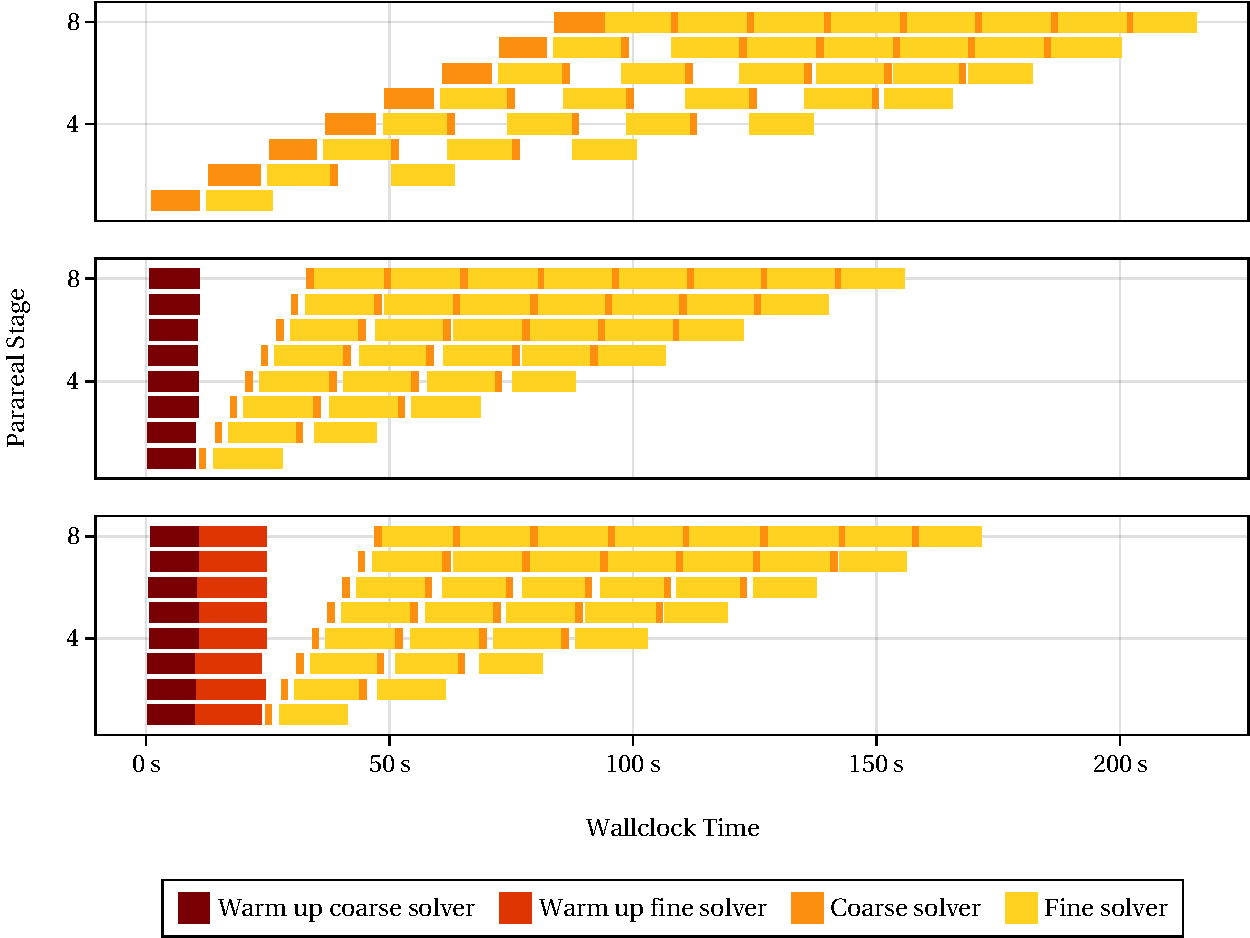
\includegraphics[width=\textwidth]{figures/fig_impl_warmup1.pdf}%
    \renewcommand\thefigure{7.1} % number in thesis
    \caption{Timeline charts}
    \lstinline!bash fig:impl:warmup.job!
    \end{figure}
  \column{0.35\textwidth}
    \begin{itemize}
      \item
        No warm-up:\\ sequential compilation
        \vspace{2em}
      \item
        Warming-up $G$:\\ parallel compilation
        \vspace{2em}
      \item
        Warming-up $F,G$:\\ no further benefit
        \vspace{2em}
      \pause
      \item[$\leadsto$]
        Always warm-up $G$\\ and $G$ only
    \end{itemize}
    \vspace{2em}
  \end{columns}
\end{frame}

\begin{frame}[t]{Estimating Parareal Runtime}
  \begin{block}{Runtime Model}
  \begin{equation*}
    \hattpar
    := \twarmup
    + \underbrace{
      \strut
      N \cdot (\trampup + t_G)
    }_{\substack{
      \text{stages $1\leq n\leq N$}\\
      \text{refinement $k=0$}
    }}
    + \underbrace{
      \strut
      K \cdot (t_F + t_G)
    }_{\substack{
      \vphantom{\text{stage}}
      n = N \\
      1 \leq k \leq K
    }}
    + t_F
  \end{equation*}
  \end{block}
  \only<1>{%
  \begin{figure}
    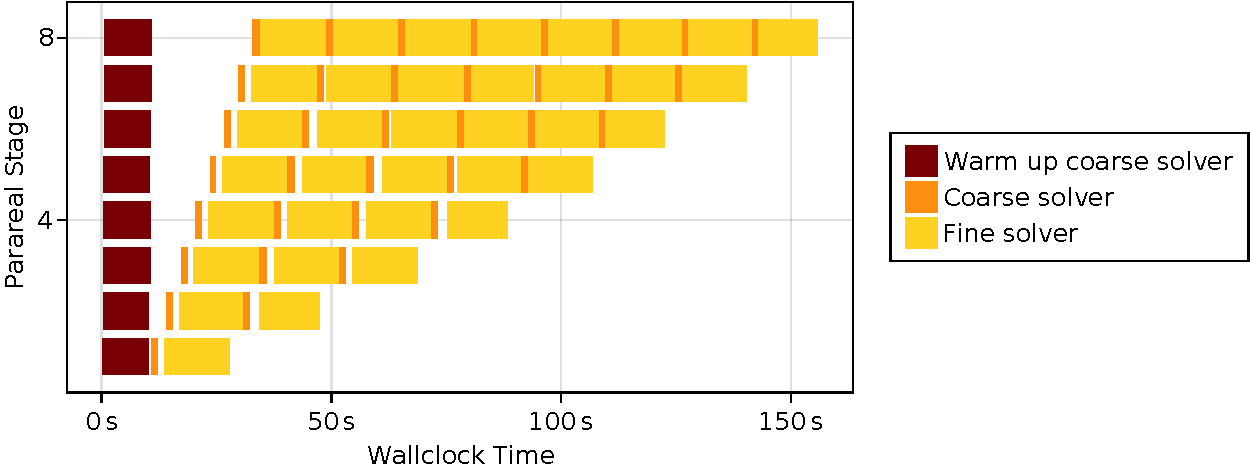
\includegraphics[width=0.7\textwidth]{figures/slides_timeline8.pdf}
    \caption{Timeline of $N=8$ stages computing $K=7$ refinements}
  \end{figure}}
  \only<2>{%
  \begin{table}
    \small
    \begin{tabular}{%
      lcc
      S[table-format=2.2]
      S[table-format=2.2]
      S[table-format=1.2]
      S[table-format=2.2]
      S[table-format=3.2]
      S[table-format=3.2]
      S[round-precision=3, round-minimum=0.001, table-format=<1.3, scientific-notation=fixed, fixed-exponent=0] % err
    }
      \toprule
      {warm-up} &
      {$N$} &
      {$K$} &
      {$\twarmup$} &
      {$\trampup$} &
      {$t_G$} &
      {$t_F$} &
      {$\tpar$} &
      {$\hattpar$} &
      {$\abs*{\frac{\hattpar-\tpar}{\tpar}}$} \\
      \midrule
      none & 8 & 7 & 0.0 & 10.448182003838676 & 1.3971984386444092 & 13.686557531356812 & 215.85136604309082 & 214.03589286123002 & -0.008410756045427896 \\
$G$ & 8 & 7 & 10.995897054672241 & 1.7753152676991055 & 1.3795734643936157 & 14.053897976875305 & 155.979896068573 & 158.32320497717177 & 0.015023147005871765 \\
$G$ and $F$ & 8 & 7 & 24.658120155334473 & 1.805815781865801 & 1.3864995241165161 & 13.99841558933258 & 171.88022804260254 & 171.88946398666928 & 5.373476735471789e-5 \\

      \bottomrule
    \end{tabular}
  \end{table}
  \begin{itemize}
    \item $t_F, t_G$: median runtime
    \item $\twarmup$: maximum runtime
    \item $\trampup$: mean delay between adjacent $G(U^0_*)$ minus $t_G$
  \end{itemize}
  }
\end{frame}
